\section{Iris Recognition}
\label{sec:Iris_Recognition_Research}
Modern iris recognition was first introduced in an article by \cite{Daugman1993} discussing the security of using iris for recognition. Here an outline of how to do recognition was laid out and even though the field has been extensively \todo{extensively what?} since, the general methodology is more or less the same as Daugman proposed. A modern system is typically composed of image acquisition, segmentation and normalisation, feature extraction and matching. 

\subsection{Images}
The images acquired are often taken in the \gls{nir} spectrum, which is ranging between 700 nm and 900 nm in wavelength. In this band, the melanin in the iris, which is the substance that gives the iris its colour e.g. brown or blue, is typically less prominent making the unique structure in the iris very distinct. To acquire usable \gls{nir} images, the user has to be in the millimetre range of the \gls{nir} camera. In the visible light, the melanin is much more prominent and thus makes is harder to detect the structure. The band of visible light has many names in the literature, namely Visible Spectrum (VIS), Visible Wavelength (VW), and \gls{vl}. \gls{vl} will be used in this report. While \gls{nir} is beneficial in some cases, other useful features can be observed in the \gls{vl} that cannot be seen with \gls{nir}. These can include the moles, freckles and conjunctival vasculature, which can help in making more accurate recognition systems. To make iris recognitions systems comparable with each other some publicly available databases are often used. \cite{Rifaee2017}  give an outline of the some of the free databases that are used. A comprehensive table summarising the visual properties, statistics and type of subject used in various database are tabulated in \autoref{fig:Iris_database_1} and \autoref{fig:Iris_database_2}. Most of the databases available are \gls{nir} images with CASIA being one of the most used database. For \gls{vl} images, UBIRIS in the most commonly used. These contain more "real world" data as the images contain more noise in the form of eyelids obstruction, eyelash obstruction, glare, motion blur, out-of-focus or poor focused iris, partial iris and specular reflection \citep{Rattani2017}. The database has also been used in Noisy Iris Challenge Evaluation (NICE) I. The increasing usage of mobile devices also proposes an opportunity to integrate iris recognition as a biometric for verifying the identity of the user. For this purpose a competition, Mobile Iris CHallenge Evaluation (MICHE), is made to compare the state of the art mobile iris. They provide a the MICHE database that can be used, which they claim is a better database than UBRIS for mobile systems. The database contains noisy iris images taken with a Galaxy Samsung IV, iPhone 5, and Galaxy Tablet II. The noise includes noise from both artificial and natural light sources during acquisition, motion blur, occlusion due to eyelids, glasses, eyelashes, hair, or shadows, which can naturally occur when a user is trying to unlock a phone using their iris. 

\begin{figure}[H]
\centering
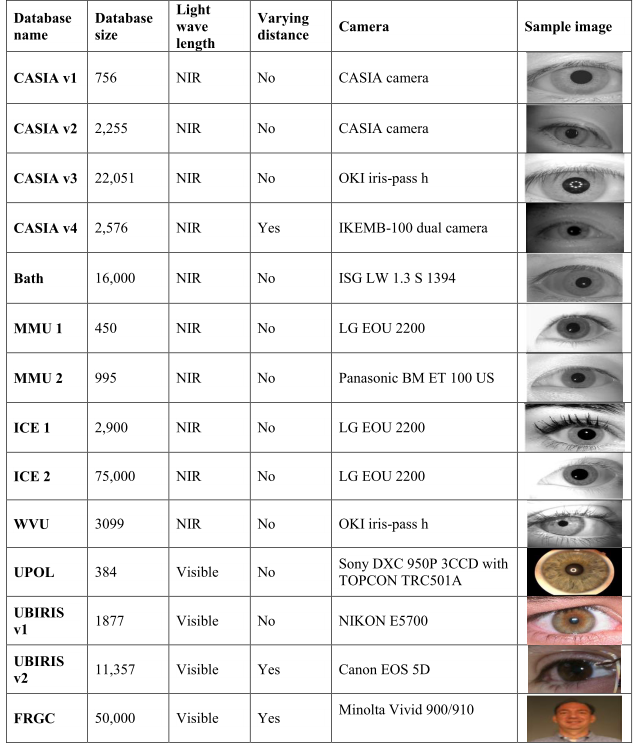
\includegraphics[width=\textwidth]{figures/Iris_Database_tabel_1.png} 
\caption{A table depicting the contents of free iris image databases  \citep{Rifaee2017}.}
\label{fig:Iris_database_1}
\end{figure}

\begin{figure}[H]
\centering
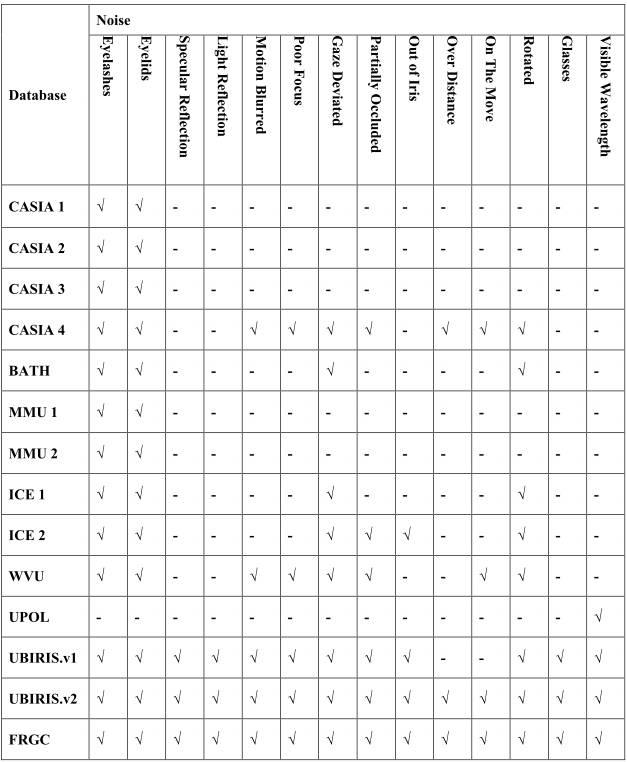
\includegraphics[width=\textwidth]{figures/Iris_Database_tabel_2.png} 
\caption{A table depicting the noise present in the databases  \citep{Rifaee2017}.}
\label{fig:Iris_database_2}
\end{figure}


\subsection{Segmentation}
Segmentation of an iris in iris recognition systems tries to detect the iris and find the pupillary boundary and the limbus boundary as well the eyelids and eyelashes that can cause noise on the image. The boundaries along with other parts of the iris can be seen in \autoref{fig:iris_naming}. The approach used for segmentation depends among other things on the wavelength of the image; \gls{nir} or \gls{vl}. They both have some common challenges to them. Often the eyelids can cover a small part of the iris, causing the limbus boundary of the iris to not be circular or elliptical. Eyelashes can also cause a similar disturbance as they also can cover parts of the iris. Poor lighting can also make it extremely difficult to detect the boundaries. Specular reflections in the iris can also cause difficulties as they can lie on the iris boundary or close to. Most systems also require a great deal of user cooperation as an off angle iris, motion blur, or glasses or contact lenses can make it even more difficult to detect the boundaries. This can especially be the case for iris recognition in a phone as it cannot be expected of the user knows how to acquire a good iris image. 

\begin{figure}[H]
\centering
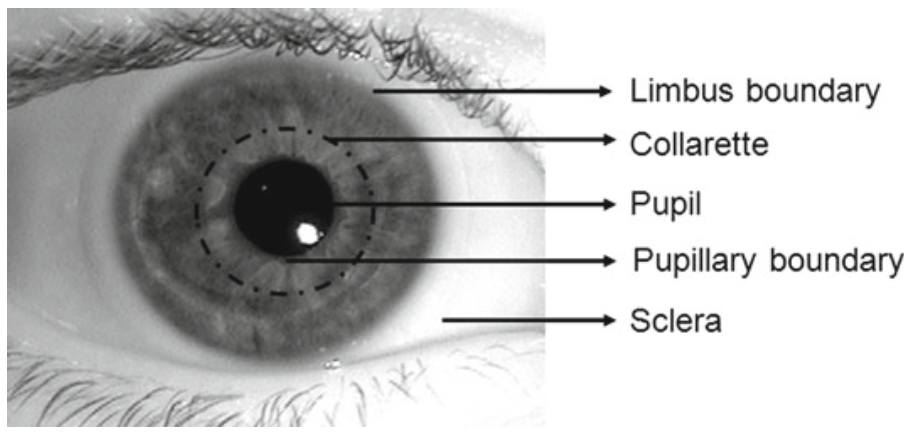
\includegraphics[width=\textwidth]{figures/iris_naming.png} 
\caption{A close up \gls{nir} image of an iris depicting the different parts of the iris along with their names \citep{Bowyer2016b}}
\label{fig:iris_naming}
\end{figure}

Two commonly observed approaches for segmentation in \gls{nir} band images are Daugman's approach \citep{Daugman1993} , \citep{Saha2017}, \citep{Rattani2017}, \citep{Khan2017}, and Hough Transform \citep{Luhadiya2017}, \citep{Uka2017}. Daugman's approach consists of using a Gaussian filter on the image to attenuate the effect of noise and eliminate undesired weak edges like the boundaries within the iris while keeping the strong edges like iris boundaries and eyelid boundaries. An integro-differential operator is then used as a circular edge detector. It is then used iteratively to find the pupillary boundary and the limbus boundary. Hough Transform on the other hand is a histogram based model fitting approach. An edge map of the input map is generated using a gradient-based edge detector. Then a voting procedure is applied on the thresholded edge map to determine the parameters for a contour that best fits a circle. This operation gives an approximate edge map of the iris boundary. Lastly, the segmented iris is often normalised using Daugman's rubber sheet model that maps every point in the segmented region from cartesian to polar coordinates. An open source MATLAB implementation based on updated version of the Daugman approach is a commonly used tool\todo{Remember to add a proper citation}. There exist other methods for different circumstances, but these are two most commonly used. They can also be used on \gls{vl} images if the image is converted from RGB to grey scale images \citep{Bowyer2016b} \todo{How to properly cite a book where each chapter is written by different people?}. 

\subsection{Feature extraction and classification}
There are multiple ways that the features can be extracted from the segmented iris. The most commonly used in the literature is a 2D Gabor filter which is a linear filter used for edge detection \citep{Daugman1993}. The Hamming distance is then used as way to classify the iris. The Hamming distance is a measurement of how many bit flips a piece of data need to have to match another piece of data. The bits of the extracted features are then measured against the whole database and the pair with the lowest score is a match. This is called "1-to-N search". As the database gets larger and larger the computation time also grows as it will have to search through the whole database. That's why \cite{Kuehlkamp2016} have suggested using a "1-to-first search" instead to improve the speed of the search. Here a threshold is chosen and as soon as a match has been found below the threshold it will stop the search. Other approaches to the categorisation have been proposed using machine learning. \cite{Khan2017} proposed using \gls{svm}, \gls{knn} and \gls{lda} with respective test accuracies of 97\%, 95.1\%, 94.28\%. In comparisons the  commercial systems ranged from 94.57\% to  99.67\% with VeriEye having the lowest and IriCore having the highest accuracy. 

\subsection{Deep Learning}
According to \cite{Zhao2017a} research in neural networks within iris recognition is still very new and not much has been done. Some of the work that has been done have used \gls{cnn} and a \gls{dbn}. \cite{Al-Waisy2017} used a common \gls{cnn} to extract features and classify a segmented and normalised iris image. The segmentation was done using Circular Hough Transform (CHT) normalisation was done using Daugman's rubber sheet method. They named the network IrisConvNet and the architecture was inspired by the Spoofnet \todo{maybe add a source or explanation if needed?}  as it can be seen in \autoref{fig:Al_Waisy2017_CNN_model}. This was the general architecture and they tried different numbers of maps and layers to find the best architecture. In general a 3x3 input kernal was used on a 64x64 or 128x128 pixel input image to create feature maps followed by 2x2 max pooling, 5x5 convolution, 2x2 max pooling 5x5 convolution, 2x2 max pooling, 5x5 convolution and finally a two fully connected layers to to a softmax regression classifier layer. A ReLU activation function is applied on the top of the convolutional and fully connected layers because it results in several times faster training without sacrificing accuracy. The AdaGrad algorithm was used for training the network. Three databases were used; SDUMLA-HMT, CASIA-Iris-V3 and IIT Dehli (IITD). IrisConvNet scored an accuracy of 99.82\% at categorising CASIA-Iris-V3 in 0.65 s. architecture 

\begin{figure}[H]
\centering
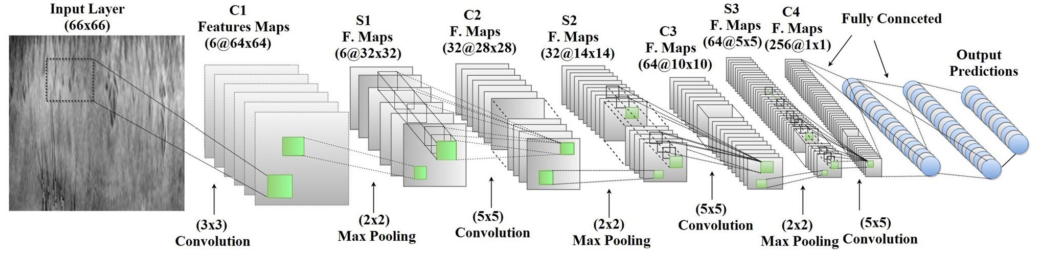
\includegraphics[width=\textwidth]{figures/Al_Waisy2017_CNN_model.png} 
\caption{Example of a \gls{cnn} architecture  from \cite{Al-Waisy2017}.}
\label{fig:Al_Waisy2017_CNN_model}
\end{figure}


\cite{Zhao2017a} claim that the problem with traditional networks are that they are database specific and not very generalisable. They created a \gls{fcn} using a loss function they created specifically for iris networks called Extended Triplet Loss (ETL). They claim this network is more generalisable than the previous networks and it shows superior results compared with IrisCode\todo{IrisCode? what is this?} which is Daugman's segmentation and normalisation approach. A \gls{fcn} differs from a \gls{cnn} in that there are no fully connected layers, only convolutional layers, max pooling etc. They proposed an architecture called UniNet that can be seen in \autoref{fig:Zhao2017_CNN_model}. It consists of two \gls{fcn}s; FeatNet and MaskNet. The network takes an iris that has been segmented and normalised using a recent approach \citep{Zhao2015a}. The segmented iris has a resolution of 64x512 pixels. The image is then fed through FeatNet and MaskNet. FeatNet extracts the iris features while MaskNet masks the non-iris part of the image. e.g an eyelid that occludes.  Three of these UniNet networks are then trained in parallel in Triplet-based network architecture that uses the ETL loss function. They used four databases to train and the networks; ND-IRIS-0405, CASIA V4, IITD and WVU Non-ideal Iris Database. It was then compared with a \gls{cnn} network based on VGG-16 that used softmax, \gls{cnn} with triplet, FeatNet only and DeepIrisNet which is a \gls{cnn} that is proposed directly for iris recognition. The results can be seen in \autoref{fig:Zhao2017_CNN_results} where UniNet outperforms the other nets and FeatNet is the by far worst performing network, which suggests that MaskNet is needed for the network to perform well. 

\begin{figure}[H]
\centering
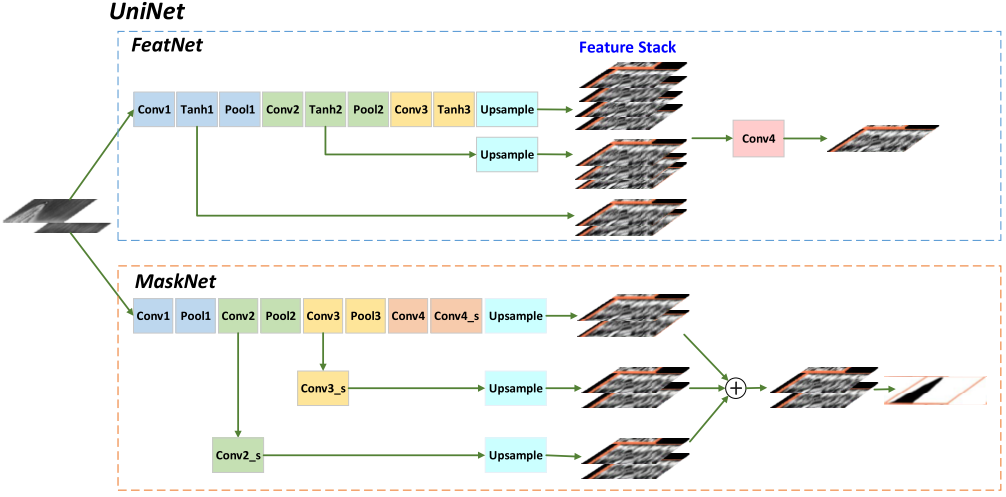
\includegraphics[width=\textwidth]{figures/Zhao2017_CNN_model.png} 
\caption{Example of a \gls{cnn} architecture  from \cite{Zhao2017}.}
\label{fig:Zhao2017_CNN_model}
\end{figure}

\begin{figure}[H]
\centering
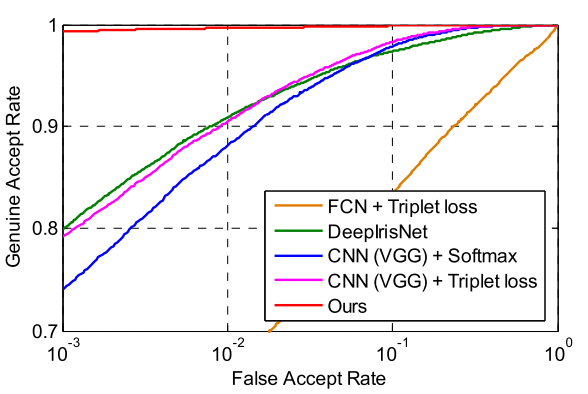
\includegraphics[width=\textwidth]{figures/Zhao2017_CNN_results} 
\caption{Results from the different networks tested on the ND-IRIS-0405 database  \cite{Zhao2017}. "Ours" is UniNet and FCN + Tripletloss is FeatNet}
\label{fig:Zhao2017_CNN_results}
\end{figure}


Another promising approach by \cite{Bazrafkan2017} targets iris segmentation in low-quality consumer images obtained from smartphones is using \gls{spdnn} for generating iris maps from low quality iris images.  In \gls{spdnn} several deep networks are merged into a single model. This way it is possible to include different networks designs and combine their strengths. They combined four \gls{fcn}s of different architectures that used a variaty of kernel sizes and layers. An example of one of the \gls{fcn}s has 12 convolutional layers  in this order; 3x3,5x5,7x7,9x9,11x11,13x13,15x15,13x13,11x11,9x9,7x7,5x5 and an output layer that is 3x3.It was trained by using the databases Bath800, CASIA Thousand, UBRIS and MobBio. They contained both \gls{nir} and \gls{vl}\todo{consider whether it makes sense to call it VL images rather than RGB images} images. Extensive noise was also added to the training images in the form of blur and lower contrast to generate degraded versions of the high quality images and utilise the databases better by creating more samples. Using the UBRIS database as a comparison with other state of the art segmentation techniques it achieved the highest accuracy with 99.30\%. The technique with the lowest accuracy, of the ones it was compared to, had an accuracy of 98.10\%.   









%\cite{Rifaee2017} gives an outline of commercially free databases often used in research.\autoref{fig:Iris_database_1} and \autoref{fig:Iris_database_2} show the different contents of the databases. Most of the databases are \gls{nir} images with CASIA being one most used databases in the literature.  For images in the visible light UBRIS is often used . These contain more "real world" data as the images contain more noise in the form of eyelids obstruction, eyelash obstruction, glare, motion blur, out-of-focus or poor focused iris, partial iris and spec- ular reflection \citep{Rattani2017}. The database has also been used in Noisy Iris Challenge Evaluation (NICE) I. For iris recognition system on mobile platforms the Mobile Iris CHallenge Evaluation (MICHE) database can be used.  The database contains noisy images taken withe Galaxy Samsung IV, Iphone5 and Galaxy Tablet II. The noise includes noise from both artificial and natural light sources during acquisition, motion blur, occlusion due to eyelids/glasses/eyelashes/hair/shadows which can naturally occur when a user is trying to unlock a phone using their iris. 


%. It was also the foundation for IrisCode which is a commercially developed iris recognition algorithm by John Daugman. In 2016 a handbook for iris recognition by \cite{Bowyer2016b} was published giving an outline of the whole process of iris recognition. In general Near Infra-Red (NIR) images of an iris are used but other type of images can also be used.  \cite{Khan2017a} show how to use Daugmans methodology on iris images taken with a smartphone in visible light. They use Daugmans Integro-differential operator to localise the bounds of the iris. Then they suppress the eyelids the eyelids which often cover parts of the iris by using an approach inspired by Masek. Afterwards the image is normalised by using the homogeneous rubber sheet model by Daugman. Then eyelashes are removed from the image and feature extraction is done by using 2D Gabor Waveletts. This approach to extract features in one way or another can be seen in multiple state of the art iris recognition systems and research papers e.g \citep{Luhadiya2017a,Uka2017a,Kuehlkamp2016a}, \cite{Kuehlkamp2016a}. After the features have been extracted they are compared/categorised. Traditionally a "1-to-N search" has been done. Here the Hamming distance of features of the scanned iris are compared to the whole database and it is classified with the iris that has the least distance. \cite{Kuehlkamp2016a} have suggested using a "1-to-first search" instead to improve the speed of the search. Here a threshold is chosen and as soon as a match has been found below the threshold it will stop the search. Other approaches to the categorisation have been proposed using machine learning. \cite{Khan2017a} proposed using Support Vector Machines (SVM), K-Nearest-Neighbours(KNN) and Linear Discriminant Analysis (LDA) with respective test accuracies of 97\%, 95.1\%, 94.28\%. \cite{Zhao2017b} proposed using deep learning to classify. They claim that research in neural networks with iris recognition is still very new and not much has been done. But some of the work that has been done have used Convolutional Neural Networks (CNN) and a Deep Belief Network (DBN). They claim that the problem with traditional networks are that they are very database specific on not very generalisable. \cite{Zhao2017b} created a Fully Convolutional Network (FCN) using a loss function they created specifically for iris networks called Extended Triplet Loss (ETL). They claim this network is more generalisable than the previous networks. 




